\documentclass{article}%
\usepackage[T1]{fontenc}%
\usepackage[utf8]{inputenc}%
\usepackage{lmodern}%
\usepackage{textcomp}%
\usepackage{lastpage}%
\usepackage{graphicx}%
\usepackage{float}%
\usepackage{tikz}%
\usepackage{pgfplots}%
%
\title{Beam Engineering Report}%
\author{Auto Generated}%
\date{\today}%
%
\begin{document}%
\normalsize%
\pgfplotsset{compat=1.18}%
\maketitle%
\section{Introduction}%
\label{sec:Introduction}%
This report is generated from Excel beam result data.%
\newline Beam Span: 15.00 m%


\begin{figure}[H]%
\centering%
\includegraphics[width=0.8\textwidth]{beam.png}%
\caption{Simply Supported Beam}%
\end{figure}

%
\section{Excel Table}%
\label{sec:ExcelTable}%
\begin{tabular}{|c|c|c|c|}%
\hline%
Start&End&Shear Force&Bending Moment\\%
\hline%
0.00&&45.00&0.00\\%
\hline%
1.50&&36.00&60.75\\%
\hline%
3.00&&27.00&108.00\\%
\hline%
4.50&&18.00&141.75\\%
\hline%
6.00&&9.00&162.00\\%
\hline%
7.50&&0.00&168.75\\%
\hline%
9.00&&{-}9.00&162.00\\%
\hline%
10.50&&{-}18.00&141.75\\%
\hline%
12.00&&27.00&108.00\\%
\hline%
13.50&&{-}36.00&60.75\\%
\hline%
15.00&&{-}45.00&0.00\\%
\hline%
\end{tabular}

%
\section{Diagrams}%
\label{sec:Diagrams}%

\begin{center}
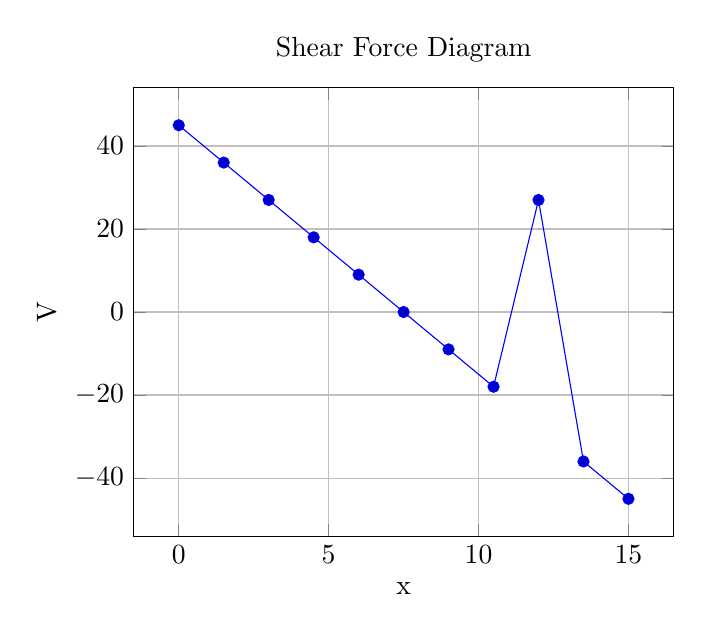
\begin{tikzpicture}
\begin{axis}[
title=Shear Force Diagram,
xlabel=x,
ylabel=V,
grid=both]
\addplot coordinates {(0.0000,45.0000) (1.5000,36.0000) (3.0000,27.0000) (4.5000,18.0000) (6.0000,9.0000) (7.5000,0.0000) (9.0000,-9.0000) (10.5000,-18.0000) (12.0000,27.0000) (13.5000,-36.0000) (15.0000,-45.0000)};
\end{axis}
\end{tikzpicture}
\end{center}
%

\begin{center}
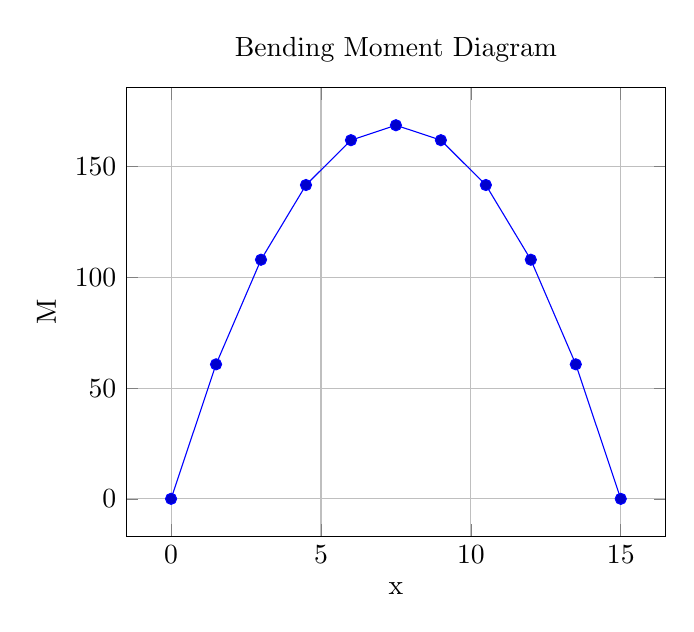
\begin{tikzpicture}
\begin{axis}[
title=Bending Moment Diagram,
xlabel=x,
ylabel=M,
grid=both]
\addplot coordinates {(0.0000,0.0000) (1.5000,60.7500) (3.0000,108.0000) (4.5000,141.7500) (6.0000,162.0000) (7.5000,168.7500) (9.0000,162.0000) (10.5000,141.7500) (12.0000,108.0000) (13.5000,60.7500) (15.0000,0.0000)};
\end{axis}
\end{tikzpicture}
\end{center}

%
\end{document}